\documentclass{article}
\usepackage[utf8]{inputenc}
\usepackage{enumitem}
\usepackage{amsmath}
\usepackage{algorithm}
\usepackage[noend]{algpseudocode}
\usepackage[margin=1.25in]{geometry}
\usepackage{pdfpages}

\usepackage{listings}
\usepackage{color}
\usepackage{graphicx}


\definecolor{codegreen}{rgb}{0,0.6,0}
\definecolor{codegray}{rgb}{0.5,0.5,0.5}
\definecolor{codepurple}{rgb}{0.58,0,0.82}
\definecolor{backcolour}{rgb}{0.95,0.95,0.92}
 
\lstdefinestyle{mystyle}{
    backgroundcolor=\color{backcolour},   
    commentstyle=\color{codegreen},
    keywordstyle=\color{magenta},
    numberstyle=\tiny\color{codegray},
    stringstyle=\color{codepurple},
    basicstyle=\footnotesize,
    breakatwhitespace=false,         
    breaklines=true,                 
    captionpos=b,                    
    keepspaces=true,                 
    numbers=left,                    
    numbersep=5pt,                  
    showspaces=false,                
    showstringspaces=false,
    showtabs=false,                  
    tabsize=2
}


\lstset{
  tabsize=4,
  language=c++,
  style = mystyle
}

\title{CS352 (Winter 2018) - Homework 5}
\author{Marc Tibbs (tibbsm@oregonstate.edu)}
\date{Due Date: February 18, 2018}

\begin{document}

\maketitle

\noindent \textbf{Problem 1:} \textit{(3 points)} \\

\noindent \textbf{Demonstrate Prim's algorithm on the graph below by showing the steps in subsequent graphs as shown in Figures 23.5 on page 635 of the text. What is the weight of the minimum spanning tree? Start at vertex a.}
\\[.25cm]

\noindent The weight of the minimum spanning tree is 32. Please see Appendix A for the graphs showing the steps Prim's algorithm would take.
\\[.25cm]

\noindent \textbf{Problem 2:} \textit{(6 points)} \\

\noindent \textbf{Consider an undirected graph G=(V,E) with nonnegative edge weights w(u,v)$\geq$0. Suppose that you have computed a minimum spanning tree G, and that you have also computed shortest paths to all vertices from vertex s$\in$V. Now suppose each edge weight is increased by 1: the new weights w'(u,v) = w(u,v) + 1.}
\\[.25cm]

\noindent \textbf{(a) Does the minimum spanning tree change? Give an example it changes or prove it cannot change.}
\\[.25cm]
The minimum spanning tree would not change. Since the all weights are increased by the same amount, Prim's algorithm would still traverse the tree in the same order and the same minimum spanning tree would be created with the new weights. Consider a graph with vertices A, B, C, and D. The edge weight for AB = 1, AC = 2, CD = 3, DB = 4. Starting from A the minimum spanning tree would be created by (1) Adding AB to the tree (2) adding AC (3) adding CD. If you added one to each edge weight the minimum spanning tree would be created in the exact same manner since AB $<$ AC $<$ CD $<$ DB still holds true. 
\\[.25cm]

\noindent \textbf{(b) Do the shortest paths change? Give an example where they change or prove they cannot change.}
\\[.25cm]
The shortest path might change after a change in the edge weights. Consider a graph with vertices A, B, C, and D. The edge weight for AB = 1 and the edge weights for AC, CD, and DB = 0. The shortest path for this graph then is A, C, D, B. However, if all weights were increased by one so that AB = 2, and AC, CD, and DB = 1, then the shortest path for the graph would be A, B and not A, C, D, B. 
\\[.25cm]
\\

\noindent \textbf{Problem 3:} \textit{(4 points)} \\

\noindent \textbf{In the bottleneck-path problem, you are given a graph G with edge weights, two vertices s and t and a particular weight W; your goal is to find a path from s to t in which every edge has at least weight W.}
\\[.25cm]

\noindent \textbf{(a) Describe an efficient algorithm to solve this problem.}
\\[.25cm]
There are two approaches for this problem. If you are simply looking for any path between the vertices s and t, then you could use a modified version of a BFS algorithm that ignored all edges with weights less than W. However, if you are looking for the shortest path between the two vertices, you would have to use a modified version of Dijkstra's algorithm that ignores all edges with weights less than W. Since the question does not specify shortest path, I will only show the modified pseudocode for the BFS algorithm.
\\[.25cm]
\textbf{BFS(G,s)} \{ \\
\indent initialize vertices;\\
\indent Q = \{s\};\\
\indent while(!Q.empty()) \{ \\
\indent\indent u = DEQUEUE(Q);\\
\indent\indent for each v $\in$ G.Adj[u] \{ \\ 
\indent\indent\indent if (v.color == WHITE \&\& distance between u and v $\geq$ W) \{ \\
\indent\indent\indent\indent v.color = GREY;\\
\indent\indent\indent\indent v.d = u.d+1;\\
\indent\indent\indent\indent v.p = u;\\
\indent\indent\indent\indent ENQUEUE(Q, v)\\
\indent\indent \} \\
\indent\indent u.color = BLACK;\\
\indent \} \\
\} \\


\textbf{(b) What is the running time of your algorithm?}
\\[.25cm]
The running time of the algorithm to find a path between s and t would be $\mathcal{O} (E + V)$ using a modified version of a BFS algorithm. If you are interested in finding the shortest path in between the to vertices, then you would need to use Dijkstra's algorithm so the runtime would be $\mathcal{O} (E\ lg \ V)$.
\\[.25cm]

\noindent \textbf{Problem 4:} \textit{(5 points)} \\

\noindent \textbf{Below is a list of courses and prerequisites for a factious CS degree.}
\\[.25cm]

\begin{center}
 \begin{tabular}{||c | c||} 
 \hline
\textbf{Course} & \textbf{Prerequisite} \\ 
 \hline\hline
 CS 150 & None  \\ 
 \hline
 CS 151 & CS 150  \\ 
 \hline
  CS 221 & CS 151  \\ 
 \hline
  CS 222 & CS 221  \\ 
 \hline
  CS 325 & CS 221  \\ 
 \hline
  CS 351 & CS 151 \\ 
 \hline
  CS 370 & CS 151  \\ 
 \hline
  CS 375 & CS 151, CS 222  \\ 
 \hline
  CS 401 & CS 375, CS 351, CS 325, CS 222 \\ 
 \hline
  CS 425 & CS 325, CS 222 \\ 
 \hline
    MATH 200 & None  \\ 
 \hline
   MATH 201 & MATH 200  \\ 
 \hline
\end{tabular}
\end{center}


\noindent \textbf{(a) Draw a directed acyclic graph (DAG) that represents the precedence among the courses.}
\\[.25cm]
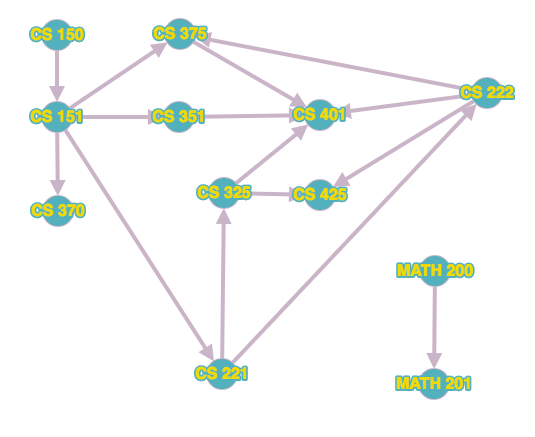
\includegraphics[scale=.75]{DAG}\\
\textbf{(b) Give a topological sort of the graph.}
\\[.25cm]
MATH 200, MATH 201, CS 150, CS 151, CS 351, CS 221, CS 375, CS 325, CS 222, CS 425, CS 401
\\[.25cm]
\textbf{(c) If you are allowed to take multiple courses at one time as long as there is no prerequisite conflict, find an order in which all the classes can be taken in the fewest number of terms.}
\\[.25cm]
Term 1: CS 150, MATH 200\\
Term 2: CS 151, MATH 201\\
Term 3: CS 370, CS 221, CS351\\
Term 4: CS 325, CS 222\\
Term 5: CS 375, CS 425\\
Term 6: CS 401\\
\\[.25cm]
\textbf{(d) Determine the length of the longest path in the DAG. How did you find it? What does this represent?}
\\[.25cm]
The longest path in the DAG is CS150, CS151, CS221, CS222, CS375, CS401 with a weight of 5. To find the longest path you need to keep track of the prerequisite class for each class. Then starting with the class with the smallest number of prerequisite classes you pop it off and record the distance it took to get there. Before you pop it off you would give the max(parent distance + 1, child distance). In this way you would get the longest paths to each vertex where the longest path represents the minimum number of steps required to list all vertices in the graph. 
\\[.25cm]

\noindent \textbf{Problem 5:} \textit{(12 points)} \\

\noindent \textbf{Suppose there are two types of professional wrestlers: "Babyfaces" ("good guys") and "Heels" ("bad guys"). Between any pair of professional wrestlers, there may or may not be a rivalry. Suppose we have n wrestlers and we have a list of r pairs of rivalries.}
\\[.25cm]

\noindent (a) Give pseudocode for an efficient algorithm that determines whether it is possible to designate some of the wrestlers as Babyfaces and the remainder as Heels such that each rivalry is between a Babyface and a Heel. If it is possible to perform such a designation, your algorithm should produce it.
\\[.25cm]

\textbf{BFS(G,s)} \{ \\
\indent initialize vertices;\\
\indent Q = \{s\};\\
\indent s.type = 'BABYFACE';\\
\indent s.d = 0;\\

\indent for each r $\in$ rivals\{\\
\indent\indent r.d = s.d + 1;\\
\indent\indent r.type = 'HEEL';\\
\indent\indent QUEUE(r);\\
\indent \}\\

\indent while(!Q.empty()) \{ \\
\indent\indent u = DEQUEUE(Q);\\

\indent\indent for each v $\in$ rivals[u] \{ \\ 
\indent\indent\indent if (v.color == WHITE) \{ \\
\indent\indent\indent\indent if (v.d $>$ u.d + 1) \{ \\
\indent\indent\indent\indent\indent v.d = u.d + 1
\indent\indent\indent\indent \} \\
\indent\indent\indent\indent if (v.d is EVEN) \} \\
\indent\indent\indent\indent\indent v.type = 'BABYFACE'
\indent\indent\indent\indent \} \\
\indent\indent\indent\indent else \} \\
\indent\indent\indent\indent\indent v.type = 'HEEL'\\
\indent\indent\indent\indent if (v.type == u.type) \} \\
\indent\indent\indent\indent\indent "Matchup not possible"\\
\indent\indent\indent\indent \} \\
\indent\indent \} \\
\indent\indent u.color = BLACK;\\
\indent \} \\


\noindent(b) What is the running time of your algorithm?\\
The running time for the algorithm would be $\mathcal{O} $(V+E) because it uses BFS. 
\\[.25cm]

\noindent(c) Implement: Babyfaces vs Heels.\\
A copy of my files including a README file that explains how to compile and run my code has been submitted in a ZIP file to TEACH.

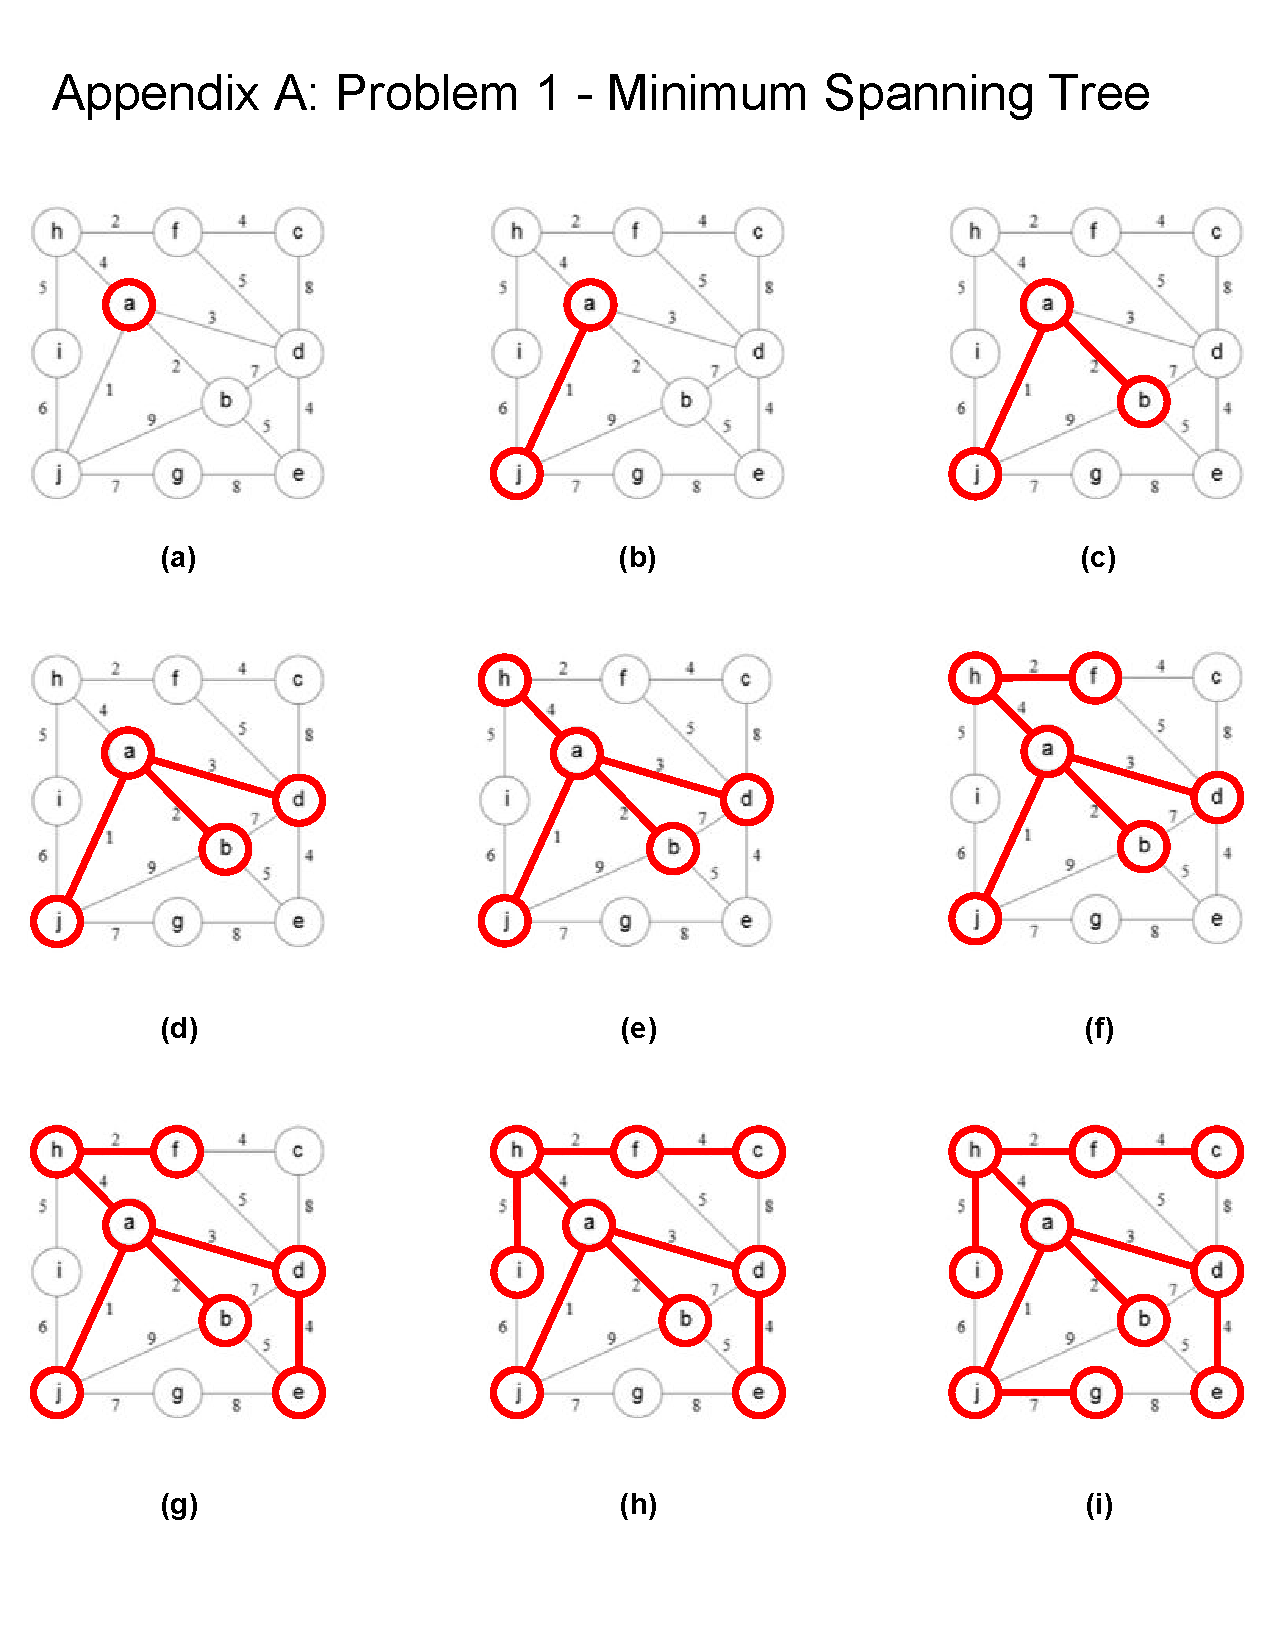
\includepdf[pages={1}]{prob1.pdf}

\end{document}
